\section{Capacitor Discharge}
CPACs 1 and 4
\hfill
\nth{11} November 2019

\subsection{Method}
\begin{enumerate}
  \item Set up the apparatus as shown in the diagram below.
  \item Press switch 1 to charge the capacitor.
  \item Press switch 3 to discharge the capacitor through G.
  \item Record the maximum deflection $\theta_1$.
  \item Press switch 1 to charge the capacitor again.
  \item Insert plug 2 fr a measured time, t seconds, to partially discharge the capacitor.
  \item Remove plug 2.
  \item Press 3 to discharge the capacitor and record the new maximum deflection $\theta_2$.
  \item Repeat with plug 2 being inserted for longer time intervals.
  \item Plot a graph of $\ln{\cfrac{\theta_1}{\theta_2}}$ against t to find C.
\end{enumerate}

\subsection{Diagram}
\begin{center}
  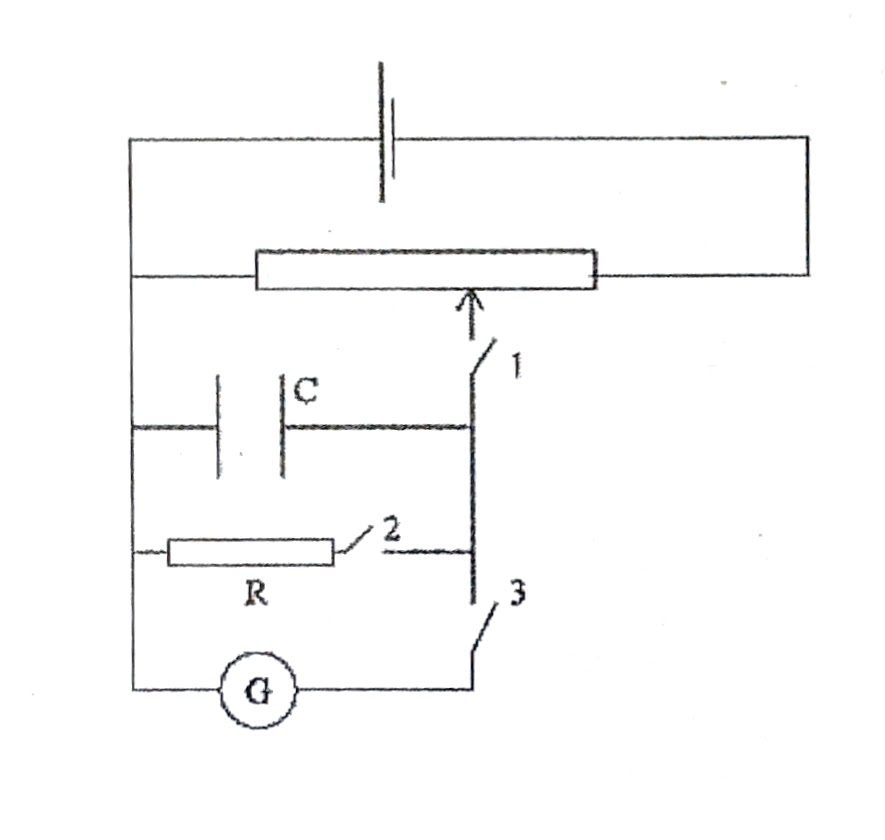
\includegraphics[width=8cm]{i_e}
\end{center}

\subsection{Results}

\begin{center}
  \pgfplotstabletypeset[
    columns={t,t1, t2, ta},
    columns/t/.style={column type = |p{1.5cm},column name= t (s)},
    columns/t1/.style={column type = |p{1.5cm}|,column name= $\theta_{n,1}$ ($^{\circ}$)},
    columns/t2/.style={column type = p{1.5cm}|,column name= $\theta_{n,2}$ ($^{\circ}$)},
    columns/ta/.style={column type = p{1.5cm}|,column name= $\theta_{n,avg}$ ($^{\circ}$)},
    string type
  ]{data/r_e.txt}
\end{center}

\subsection{Graph}

\begin{figure}[H]
  \centering
  \begin{tikzpicture}
    \begin{axis}[ylabel={Natural log of $\theta_1$ divided by $\theta_2$},xlabel={Time interval, t}]
      \addplot [mark = *] table [x=t,y=ln]{data/r_e_1.txt};
      \addplot [thick, red] table [
        x=t,
        y={create col/linear regression={y=ln, x=t}}
      ]{data/r_e_1.txt};
    \end{axis}
    \xdef\regaE{\pgfplotstableregressiona}
    \xdef\regbE{\pgfplotstableregressionb}
  \end{tikzpicture}
\end{figure}

\subsection{Analysis}
We know that the capacitance is equivalent to:
\begin{equation}
  \frac{t}{R \cdot \ln{\frac{\theta_1}{\theta_2}}}.
\end{equation}
This can be rearanged to give:
\begin{equation}
  \ln{\frac{\theta_1}{\theta_2}} = \frac{t}{C \cdot R}.
\end{equation}
Using the gradient of our graph we can conclude that:
\begin{equation}
  m = \frac{1}{C \cdot R},
\end{equation}
Which gives a capacitance of:
\begin{equation}
  C = \frac{1}{\regaE \cdot 10^6} \\
  C = 2.9 \mu F
\end{equation}

The capacitor is known to have a value of around $2\mu F$, however, as no true value was found, no comparisons can be made.

\subsection{Evaluation}
To improve this experiment a digital galvanometer should be used as there would be no error in measuring the maximum deflection. This would decrease uncertainty.

\subsection{Conclusion}
This experiment produced valid results as the value obtained was expected and in the correct order of magnitude.
